\documentclass[11pt]{article}
%\documentclass[twocolumn]{article}
\usepackage[utf8]{inputenc}
\usepackage{graphicx}
\usepackage{mathtools}
\usepackage{qtree}
\usepackage[letterpaper, top=2cm, margin=1in]{geometry}
\usepackage{listings}
\usepackage{hyperref}
\setlength{\columnsep}{0.5cm}
\usepackage{hyperref}
%\usepackage{natbib}
%\bibliographystyle{named}


\title{Relative Clauses in a Semantic Parser}
\author{Jessica Kenney}

\date{24.918 Spring 2016 Project\\\ \\
\texttt{https://github.com/seveneightn9ne/semantic-parser}}

\begin{document}

\maketitle
\tableofcontents

\section{Introduction}
This paper explores the challenges and details of implementing relative clauses as described in
Gallego (2006) in a previously existing semantic parser. The Semantic Parser system was developed
in Fall 2015 as a project for 6.S083 Computation and Linguistics.
It parsed English from text into a logical form which was then interpreted and evaluated. It then
drew conclusions or found counterexamples to conclusions in the input. The paper describing that
project is available here:
\url{https://jesskenney.com/parser.pdf}

This project builds directly from where last semester's project left off, so all improvements and
modifications on top of what is in the previous paper will be here in this paper.

\subsection{Goals}
The underlying theoretical goal of this project is to try to do things in a way the brain might do it,
 rather than in a way that is most suitable to computer programming. This means,
for example, a grammar that can parse Jabberwocky (with nonsense nouns, verbs, and adjectives) as
opposed to a grammar which uses a static dictionary. This is more computationally difficult because
the grammar allows a lot of ambiguity so there are many possible parses that have to be eliminated
by later steps. In fact, this is still an open question in linguistics in general: how is the brain
doing something that seems computationally infeasable?

The specific goal discussed in this paper is to parse relative clauses as described by Angel Gallego
in ``T-to-C movement in relative clauses". That paper was trying to provide a very thorough account
of relative clauses including phenomena that is only seen in Romance languages, not English. So the
reason for using Gallego's model is not just to be able to express English relative clauses (though
his model can express English better than the Semantic Parser's previous model), but also to evaluate
his model. By implementing it in a system that actually does semantic parsing we would verify that
the model is fairly coherent.

It is important to distinguish whether the Semantic Parser should reject ungrammatical sentences.
I think that being able to do so is interesting and very worthwhile, because it allows for a more precise theory and
model. However, theoretically it's not clear which is closer to what the human mind does. We can ``correctly" interperet
ungrammatical sentences, or at least we can glean some semantic information from them, while simultaneously
making a binary judgement that the sentence is ungrammatical. Are these two separate processes operating
on the sentence? If so, do should the Semantic Parser emulate both of them or only one? For this project,
the focus is mainly on the first, being able to translate sentences, although I use information
about how it behaves with bad sentences in order to inform the theoretical decisions of the
implementation.
% Something about being constantly a work in progress or something that sounds good but also means
% I'm not finished :) Maybe.

\subsection{Gallego's Relative Clauses}
Figures %\ref{fig:trees}
1 \& 2 show the basic structure of Gallego-style relative clauses for ``the boy who left'' and ``the boy that left" respectively.


\begin{figure}[htp]
    \centering
    \begin{minipage}{.5\textwidth}
	\centering
	\Tree [.DP [ ] [.D' [.D\\The ] [.cP' \qroof{boy}.NP$_i$ [.c' [.c\\$\emptyset$ ]
	    [.CP [.DP$_j$ [ ] [.D' [.D\\who ] [.NP\\t$_i$ ] ] ] [.C' [.C\\$\emptyset$ ]
	    [.TP [.DP$_k$\\t$_j$ ] [.T' T [.VP [.DP\\t$_k$ ] [.V' [.V\\left ] ] ] ] ] ] ] ] ] ] ]
	\caption{The boy who left}
    \end{minipage}%
    \begin{minipage}{.5\textwidth}
    	  \centering
	\Tree [.DP [ ] [.D' [.D\\The ] [.cP' \qroof{boy}.NP$_i$ [.c' [.c\\$\emptyset$ ]
	    [.CP [ ] [.C' [.C\\that$_j$ ]
	    [.TP [ ] [.T' T$_j$ [.VP [.DP [ ] [.D' [.D$_{REL}$ ] [.NP\\t$_i$ ] ] ] [.V' [.V\\left ] ] ] ] ] ] ] ] ] ] ]
	  \caption{The boy that left}
    \end{minipage}
    \label{fig:trees}
\end{figure}

The novel part of Gallego's theory is in adding this new level, cP, to which the relativized NP moves.
Some previous theories moved it to the spec of the DP, or into the spec of ForceP, but none accounted
for two facts in Romance languages: the complementizer is always required (unlike English, where ``that"
is optional in some cases) and overt relative Ds must be introduced by a preposition.

Recall that EPP, as defined by Pesetsky 2001, is a property of features which motivates movement
when the feature becomes valued via agreement.

The movement that happens in Gallego's relative clauses is motivated by a [uT, EPP] and [uRel, EPP]
feature on C, and a [u$\varphi$, EPP] feature on c. Economy of movement and the rule that ECs cannot
be pied-piped (Chomsky 2001)
combine to form this theory of relative clauses, which happens to also explain the previously exceptional
phenomena that we see in English infinitival relative clauses, where relative Ds requrie a preposition
(the same phenomena observed in Romance languages).

\section{Implementation}

\subsection{Features}
The Semantic Parser only deals with parsing text into meaning, not the other way around. Papers
introducing linguistic theories tend to write from the perspective of generating the sentence, or
going from meaning to linear text, which makes it difficult at first to see exactly what a parser's
needs are going to be. For example, feature agreement is essential when going from meaning to surface-form
tree, but is not needed nearly as much when parsing linear text to a surface-form tree. Even
semantic interpretation turns out to not require reversing movement or fully evaluating the feature
agreement used in generating the sentence.

For this reason, I started out with a lot of focus on features, as they're a core part of generating
Gallego relative clauses, even though they're nearly unnecessary in interpreting them. It turns out
that features are quite useful regardless, because they allow the grammar to be more compact (see
section 2.3 Modifications to the Grammar).

\subsubsection{Representation of a Feature}
All \texttt{Feature} types contain one field: an optional boolean value. So a feature may be
unvalued, +, or -. Each different type of feature (plural, Wh, etc.) is a subtype of \texttt{Feature}.
Each XP type determines whether an instance of that feature on that phrase will have the EPP property
(the property which causes movement when agreement occurs) and it also defines whether that feature
is intrinsic to that word (or if its value is due to agreement). So, for example, \texttt{epp(Plural, TP)}
is true because the [u$\varphi$] on T has the EPP property. Similarly, \texttt{intrinsic(Plural, NP)} is true.

In this system, features are never unvalued. Although the representation of a \texttt{Feature} allows
it, the steps from parsing to interpretation never deal with an unvalued feature. On the surface form
we see words like verbs conjugated to agree with a noun, so the grammar uses this information to value
the features when it constructs
the syntax tree. A further step of validating the feature agreement (discussed below) ensures that
the only valid trees are ones that could have been produced by a coherent agreement process.

Every XP, Xbar, and word now has a \texttt{features} field. On words, the feature set is defined
when the word is created in the grammar-based parsing step. XPs and Xbars have their features defined
recursively as the features of their head.

\subsubsection{$\varphi$-features}
$\varphi$-features are the features inherent to nouns with which verbs, determiners, etc. must agree. For
simplicity, I used only one $\varphi$-feature: Plural. Using only one $\varphi$-feature  avoids the
edge case where one agreement/movement step satisfies multiple features at once, instead of just the
feature that initiated the movement.

\subsection{New phrases, words, and structures}
\subsubsection{cP, CP, TP}
In order to represent Gallego relative clauses, we must introduce cP, CP, and TP into the Semantic
Parser. Previously, sentences were represented as simply a VP, with the subject in the spec of the VP.
Since the system always assumes simple present tense, there
wasn't much that had to be added, except allowing null heads for all three. I implemented null heads
as simply one variation of the closed class word, whose text is empty instead of the name of the word.
Note that in this model, CP is the root of a sentence, and cP is only used in relative clauses. It could
be that cP is actually the root of a sentence but that would not have any effect, because the top-level
is never relativized.

\subsubsection{DPs}
The next major change was to make DPs take NPs as a complement instead of the other way around. This
actually is helpful for the semantic interpretation step (translating from a syntax tree to a logical
structure) because the determiner determines which type of logical phrase it would be. For example,
``every dog ..." translates to $\forall x.Dog(x)\rightarrow ...$ whereas ``some dog ..." translates to
$\exists x.Dog(x) \wedge ... $. In the logical form, it's clear that the determiner scopes over the
noun semantically.

DPs now have to be able to take a cP complement as well as an NP complement. This is new for
the system, where previously a given XP type could only have one type of spec, one type of complement,
and one type of adjunct. I fixed this by redefining DP as a trait that is a subclass of \texttt{XP[Determiner, Determiner, Word, Preposition]} (so now the complement's type is not specified), and creating two
subclasses of DP: NomDP, taking a NP complement, and RelDP, taking a cP complement.

Finally, I changed pronouns to be intransitive determiners instead of nouns, because if they were
nouns there's not a clear way in the feature-agreement model to restrict them to not have some
determiner. I've disabled names/proper nouns for now, as I'll need to research more to figure out
the best way to represent them.

\subsubsection{Traces}
Because linking traces to the phrase they're a trace of is not necessary for being able to interpret
a surface phrase, I made traces very simple: they're just a null intransitive word. So for example,
a DP-trace would be represented by the structure [DP [D' [D Null$_{[\pm \text{Plural}]}$] ] ]. I
had the feeling that traces should really be replacing the whole DP, but that would be harder to
implement in the current type system because if it's a DP then it needs a spec and head, etc. So,
for simplicity, a trace is a word for now.

\subsubsection{There}
Previously, the existential ``there" (as in, ``There is a coin on the table") appeared only in the
grammar and had no representation in the syntactic structure, rather, there would be no subject
for such a sentence. However, this was slightly insufficient because to implement feature agreement,
T needs to agree with something, and EPP means there needs to be something in the spec of T which
agrees with T. So, I made There be an intransitive determiner which can have [+Plural] or [-Plural].
This way, the feature agreement works correctly and the resulting interpretation is the same.

However, this method doesn't restrict a sentence such as ``There are a man in the room" from being
interpretable. That is, there is no meaningful connection between the $\varphi$ features on There and
on the object, whereas in English they are required to agree. I didn't implement
the full solution (where the T is able to agree with the object but doesn't move it up to subject
position) because it's a pretty far digression from the original goal.

\subsection{Modifications to the Grammar}
%\label{ssec:grammar}
With the addition of features and feature agreement, the grammar can become much more compact.
Previously, enforcing feature agreement was done in the grammar, so there would be rules like:

\ \\
\indent NP $\rightarrow$ DP$_{\text{plural}}$ N'$_{\text{plural}}$ $\vert$ DP$_{\text{singular}}$ N'$_{\text{singular}}$
\ \\

This is less problematic when the only feature is [$\pm$Plural], but with the addition of more features, the
size of the grammar (measured by number of rules) grows exponentially. Consider:

\ \\
\indent NP $\rightarrow$ NP$_{\text{singular, 1person, present}}$ $\vert$ NP$_{\text{singular, 1person, past}}$ $\vert$ NP$_{\text{singular, 1person, future}}$ $\vert$ NP$_{\text{singular, 2person, present}}$ $\vert$ NP$_{\text{singular, 2person, past}}$ $\vert$ NP$_{\text{singular, 2person, future}}$ $\vert$ ...
\ \\

And this is only for the NPs, which would need to be agreeing with the VPs in the sentence as well.
Now with the addition of feature agreement as a separate step from parsing, the grammar looks much
more straightforward:

\ \\
\indent DP $\rightarrow$ DP? D' (the ? means optional)\\
\indent D' $\rightarrow$ D NP \\
\indent D $\rightarrow$ D$_{\text{plural}}$ $\vert$ D$_{\text{singular}}$
\\

Basically, all of the branching caused by features can be moved down to the leaves of the parse tree.
This means that the grammar can now output more potential parses. For example, the determiner "no"
can be singular or plural, you can't tell from just seeing it in isolation. So the grammar would output
two parses for the phrase ``no boys":\\

[DP [D' [D No$_{\text{ plural}}$ ] [NP [N' [N boys$_{\text{ plural}}$ ] ] ] ] ]\\
\indent [DP [D' [D No$_{\text{ singular}}$ ] [NP [N' [N boys$_{\text{ plural}}$ ] ] ] ] ]\\

It's up to the feature agreement validation step to eliminate the second parse.

\subsection{Transitivity \& Feature Agreement Validation}
Transitivity validation is the post-grammar process of making sure that transitive determiners (such
as ``the") have a complement, and that intransitive determiners (like ``he") don't. There is no
transitivity validation for verbs, because they're open-class, so the grammar doesn't know any verbs
and therefore doesn't know if they should be transitive or not. So this transitivity validation happens
only for DPs. Wh-determiners, such as ``who", take an NP complement, but in the surface form that NP
is always a trace (so it appears intransitive). Since we're not focusing on being able to reject bad
sentences, we mark wh-determiners as transitive and don't worry about the fact that this would allow
a DP ``who person" to be accepted. The fix for that would have to be in a trace-linking step which
does not currently exist because it's not strictly necessary for correct interpretation.

Since both feature agreement and transitivity validation require recursively walking through the
syntax tree, and return a boolean valid/invalid as a result, it should be possible to combine them
into one function. Perhaps transitivity can just be a feature on determiners, whose ``agreement"
is special-cased to mean the presence of a complement instead of a successful probe on the complement.
It's interesting to consider transitivity being just a feature, but for now the two are separate.

Feature validation has two main cases: agreement between a specifier and X', and agreement between
a head and complement. I'm ignoring adjuncts for now because I'm not sure what the rules are for
how they merge.

For agreement between a specifier YP and an X', a feature on X' which is non-intrinsic and has EPP
must have the same value as the feature resulting from a probe of YP.

For agreement between a head X and complement YP, a feature on X which is non-intrinsic and does not
have EPP must have the same value as the feature resulting from a probe of YP.

A probe is a method which searches a tree for the nearest instance of a feature and returns the value
of the feature. The T-to-C movement theory requires that specifiers and heads be equidistant, which
is what causes ``that" to be optional in English, so probe actually returns a set of features, and
the feature agreement is valid if a word agrees with any feature resulting from the probe. The probe
could fail to find any instance of the feature, and return an empty set.

After these validation steps have been run on a sentence, there are still two resulting parses: one
in which the subject sits in Spec-TP, and one in which Spec-TP is a trace and the subject sits in
Spec-VP. The validation step is unable at this point to rule out the second sentence. However,
both trees translate to the same logical form, so the system doesn't care about this ambiguity.

\section{Example}
Here is an example output parsing ``the boy who sings":

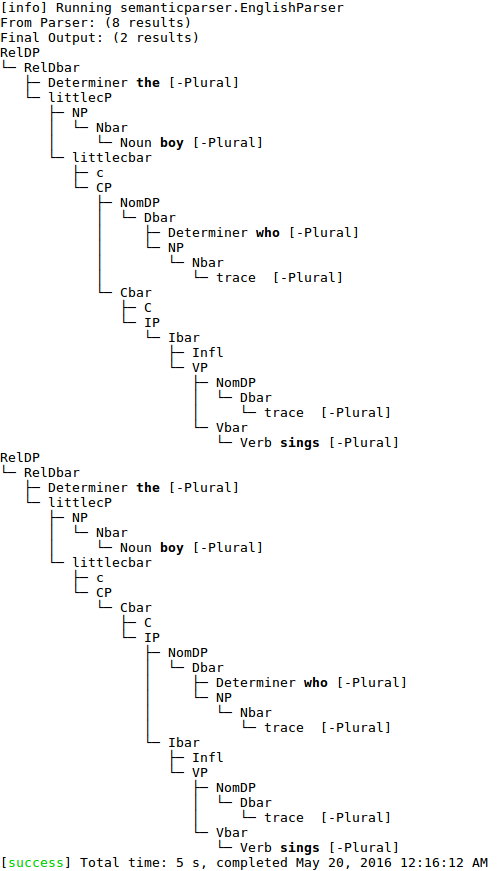
\includegraphics[width=0.6\textwidth]{trees.png}

Notice there are two valid parses because the ``who" could be in the spec of CP or TP. As explained
in section 2, this would be solved by a step that makes sure the traces are coherent.
\section{Future Work}
There are a lot of ways to go to make the system more robust. I think the most interesting thing to
do next would be to implement trace-linking which requires a much more precise understanding of the
movement that generated the sentence. However, this would also require a much more cohesive model
to implement, to account for things like ``There is a man in the house" where ``a man" is not pulled
into the subject position. This would likely require delving into phases and vP.

\section{Conclusion} % Takeaways
Implementing Gallego's relative clauses was an amazing way to learn about the details of how the
current ideas in the minimalist program work. I still think that Gallego's model has some issues.
For example, semantically it seems like the determiner which is the head of a relative clause should
be scoped under the clause, like the noun is. However, it's still a model which works very well
for my use case, and the Semantic Parser can now parse much more complex relative clauses.

\begin{thebibliography}{9}
    \bibitem{chomsky2001}
	Chomsky, Noam. 2001. ``Derivation by Phase". \emph{Ken Hale: A Life in Language},
    	ed. by M. Kenstowicz, 1-52. Cambridge, Mass.: MIT Press.
    \bibitem{gallego}
	Gallego, \'Angel J. 2006. ``T-to-C Movement in Relative Clauses". in J. Doetjes \&
	P. Gonz\'alez (eds.), \emph{Romance Languages and Linguistic Theory 2004. Selected Papers
	from ``Going Romance"} 2004, Amsterdam: John Benjamins.
    \bibitem{parse}
	Gerth, S., \& beim Graben, P. 2009. Unifying syntactic theory and sentence processing difficulty
	through a connectionist minimalist parser. \emph{Cognitive Neurodynamics}, 3(4), 297-316.
    \bibitem{ttoc}
    	Pesetsky, David, and Esther Torrego. 2001. ``T-to-C movement: Causes and consequences''.
	\emph{Ken Hale: A Life in Language}, ed. by M. Kenstowicz, 355-426. Cambridge, Mass.: MIT Press.
    \bibitem{tc}
    	Pesetsky, David, and Esther Torrego. 2002. Tense, case, and the nature of syntactic categories.
	Gu\'eron, J. \& Lecarme, J. (eds.) \emph{The Syntax of Time.} Cambridge, Mass.: MIT Press.
    \bibitem{features}
    	Pesetsky, David, and Esther Torrego. 2004. The syntax of valuation and the interpretability
	of features. \emph{Phrasal and clausal architecture: Syntactic derivation and interpretation},
	ed. by Simin Karimi, Vida Samiian, and Wendy Wilkins, 262-294. Amsterdam: John Benjamins.
    \bibitem{probes}
    	Pesetsky, David, and Esther Torrego. 2006. Probes, goals, and syntactic categories.
	\emph{Proceedings of the 7th Annual Conference on Psycholinguistics.}, ed. Y. Otsu. Keio University, Japan
    \bibitem{pulman}
	Pulman, Stephen G. 1980. ``Parsing and syntactic theory." \emph{Proceedings of the 8th conference
	on Computational linguistics} 54-59. Association for Computational Linguistics.
\end{thebibliography}
\end{document}
